\documentclass[border=3pt]{standalone}
\usepackage{fontspec}
\setmainfont{Times New Roman}
\usepackage{pgfplots}
\pgfplotsset{compat=1.18}
\usetikzlibrary{arrows.meta,calc,positioning,shapes.geometric}
\definecolor{forest}{HTML}{346E57}
\definecolor{sage}{HTML}{E8EFEA}
\definecolor{clay}{HTML}{B77E60}
\definecolor{gray}{HTML}{718078}
\definecolor{rule}{HTML}{B7C3BA}
\definecolor{ink}{HTML}{000000}
\begin{document}
\hyphenpenalty=10000\exhyphenpenalty=10000
\fontsize{10}{12}\selectfont
\renewcommand{\small}{\fontsize{9}{11}\selectfont}
\renewcommand{\scriptsize}{\fontsize{8}{10}\selectfont}
\resizebox{16cm}{!}{%
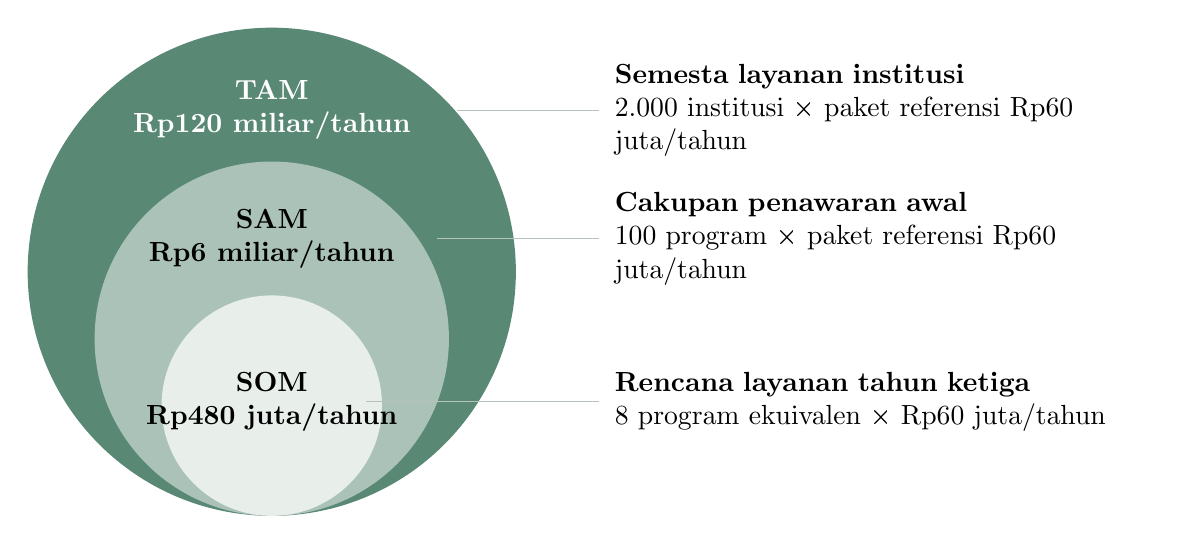
\begin{tikzpicture}[x=1cm,y=1cm]
\fill[forest!82] (0,0) circle (3.1);
\fill[forest!42] (0,-0.85) circle (2.25);
\fill[sage] (0,-1.7) circle (1.4);
\node[align=center,font=\bfseries,text=white] at (0,2.05) {TAM\\Rp120 miliar/tahun};
\draw[rule,line width=.55pt] (2.35,2.05) -- (4.15,2.05);
\node[anchor=west,align=left,text width=7cm,inner sep=0] at (4.35,2.05) {\textbf{Semesta layanan institusi}\par 2.000 institusi × paket referensi Rp60 juta/tahun};
\node[align=center,font=\bfseries,text=ink] at (0,0.42) {SAM\\Rp6 miliar/tahun};
\draw[rule,line width=.55pt] (2.1,0.42) -- (4.15,0.42);
\node[anchor=west,align=left,text width=7cm,inner sep=0] at (4.35,0.42) {\textbf{Cakupan penawaran awal}\par 100 program × paket referensi Rp60 juta/tahun};
\node[align=center,font=\bfseries,text=ink] at (0,-1.65) {SOM\\Rp480 juta/tahun};
\draw[rule,line width=.55pt] (1.2,-1.65) -- (4.15,-1.65);
\node[anchor=west,align=left,text width=7cm,inner sep=0] at (4.35,-1.65) {\textbf{Rencana layanan tahun ketiga}\par 8 program ekuivalen × Rp60 juta/tahun};
\end{tikzpicture}
}

\end{document}
